\chapter{Validación y Resultados}\label{cap:Validacion}
%Se deben incluir tantos cap\'{\i}tulos como se requieran; sin embargo, se recomienda que la tesis  o trabajo de investigaci\'{o}n tenga un m\'{\i}nimo 3 cap\'{\i}tulos y m\'{a}ximo de 6 cap\'{\i}tulos (incluyendo las conclusiones).\\

%\renewcommand{\tablename}{\textbf{Código}}

En este capítulo se pretende validar el modelo ejecutable que se realiza a partir del esquema preconceptual. Con éste propósito, se plantea un caso que se toma de \cite{jamal2006petroleum}. El cual, consiste en una simulación de un yacimiento lineal (1D) de cinco celdas con un solo fluido y un pozo productor en la cuarta celda, como se muestra en la Figura \ref{fig:Abou-Kassem} \citep{jamal2006petroleum}. Con este, se espera validar el transporte de un fluido y las pérdidas de presión por pozos.\\

El caso de estudio de \cite{jamal2006petroleum} consta de dos procesos principales, uno de pérdidas a caudal fijo, y el otro, cuando la celda perforada para el pozo alcanza la ``presión de abandono''. En este, se cambia la condición operativa del pozo para mantener la presión fija a esa presión de abandono. En la Figura \ref{fig:ConstantQ} se reportan los resultados de la simulación durante la etapa de producción a caudal constante, y en la Figura \ref{fig:ConstantP} se reportan los resultados de la simulación durante la etapa de producción a presión constante.
\begin{figure}[h]
	\centering
	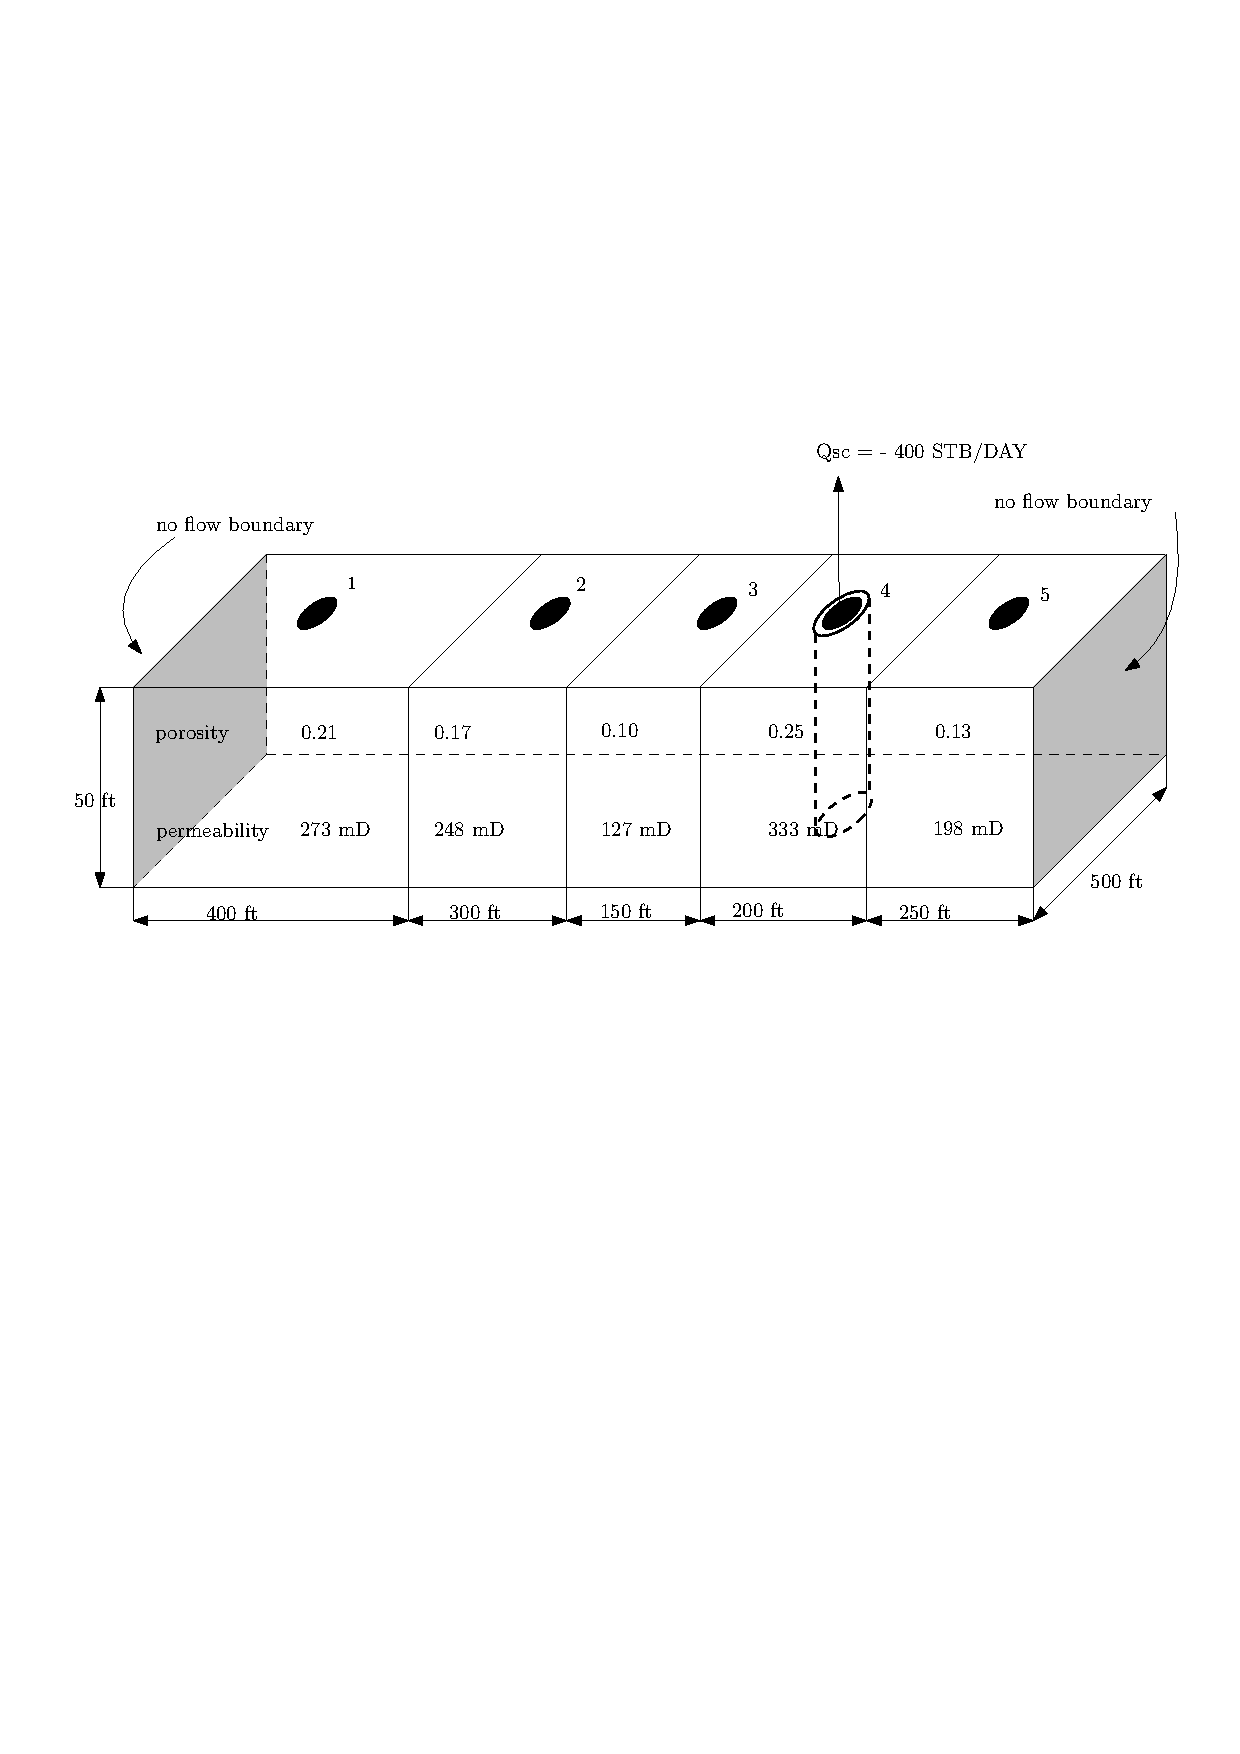
\includegraphics[width=0.9\textwidth]{Fig/casoasis.pdf}
	\caption{Representación gráfica del caso proporcionado por \cite{jamal2006petroleum}.}
	\label{fig:Abou-Kassem}
\end{figure}



\begin{figure}[h!]
	\centering
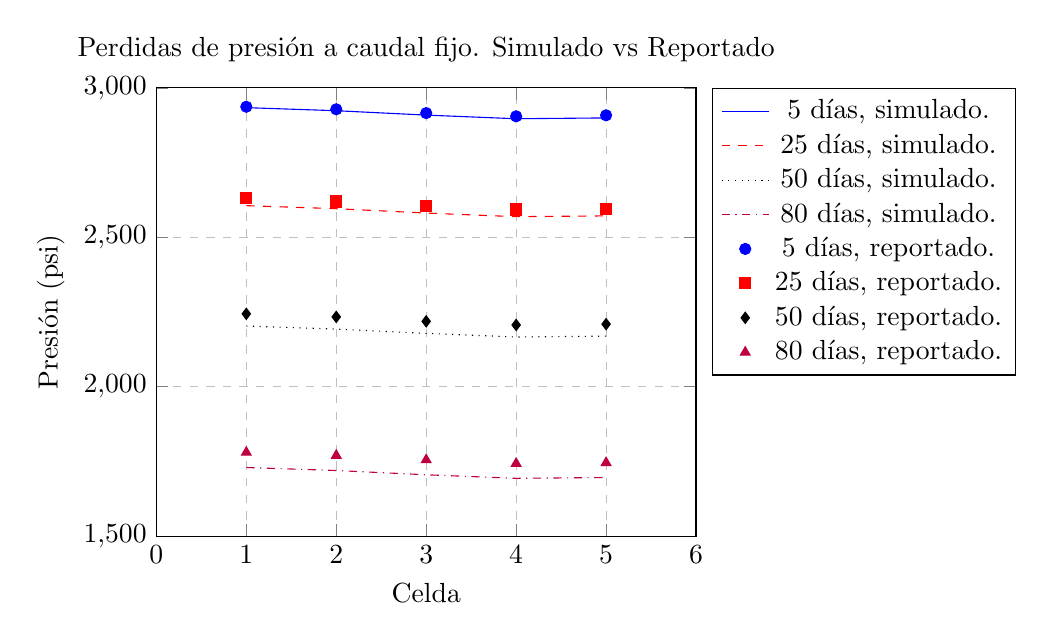
\begin{tikzpicture}
\begin{axis}[
title={Perdidas de presión a caudal fijo. Simulado vs Reportado},
xlabel={Celda},
ylabel={Presión (psi)},
xmin=0, xmax=6,
ymin=1500, ymax=3000,
legend pos=outer north east ,
ymajorgrids=true,
xmajorgrids=true,
%semilogxaxis=true,
grid style=dashed,
]

\addplot[color=blue]
coordinates{
	(1,2933.8141602)
	(2,2923.5889812)
	(3,2908.882128)
	(4,2896.698936)
	(5,2899.4836656)
	
};
\addlegendentry{5 días, simulado.}

\addplot[dashed, color=red]
coordinates{
	(1,2605.9267536)
	(2,2595.745086)
	(3,2581.1107518)
	(4,2569.0000788)
	(5,2571.741297)
	
};
\addlegendentry{25 días, simulado.}

\addplot[dotted,color=black]
coordinates{
	(1,2203.1127162)
	(2,2193.0180714)
	(3,2178.5287752)
	(4,2166.5196288)
	(5,2169.2463432)
	
};
\addlegendentry{50 días, simulado.}

\addplot[dashdotted,color=purple]
coordinates{
	(1,1729.7812032)
	(2,1719.8025888)
	(3,1705.4728344)
	(4,1693.6087260)
	(5,1696.3064328)
};
\addlegendentry{80 días, simulado.}

\addplot[only marks, mark options={draw=blue,fill=blue,}]
coordinates{
	(1,2936.80)
	(2,2928.38)
	(3,2915.68)
	(4,2904.88)
	(5,2908.18)
	
	
};
\addlegendentry{5 días, reportado.}
\addplot[only marks, mark=square*, mark options={draw=red,fill=red,}]
coordinates{
	(1,2630.34)
	(2,2620.06)
	(3,2605.28)
	(4,2593.04)
	(5,2595.81)
	
	
};
\addlegendentry{25 días, reportado.}
\addplot[only marks, mark=diamond*, mark options={draw=black,fill=black,}]
coordinates{
	(1,2243.97)
	(2,2233.68)
	(3,2218.9)
	(4,2206.66)
	(5,2209.43)
	
	
};
\addlegendentry{50 días, reportado.}
\addplot[only marks, mark=triangle*, mark options={draw=purple,fill=purple,}]
coordinates{
	
	(1,1780.3100)
	(2,1770.0200)
	(3,1755.2400)
	(4,1743.0000)
	(5,1745.7700)
	
	
};
\addlegendentry{80 días, reportado.}
\end{axis}
\end{tikzpicture}
\caption{Comparativo datos simulados contra caso de estudio de \cite{jamal2006petroleum}. Caudal constante.}
\label{fig:ConstantQ}
\end{figure}{}

Las condiciones iniciales de presión para el yacimiento son de $3000$ $psia$ para todas las celdas y el pozo se establece a una condición operativa de caudal fijo a $400$ $STB/D$. Se puede ver como en los primeros 80 días, va decayendo la presión hasta alcanzar la presión de abandono. Se encuentran diferencias entre los resultados simulados y los reportados por \cite{jamal2006petroleum} menores a $50$ $psia$. Éstas se deben, a que las ecuaciones que se implementan en el modelo ejecutable, son diferentes a las que se presentan en \cite{jamal2006petroleum}.

\begin{figure}[h!]
	\centering
	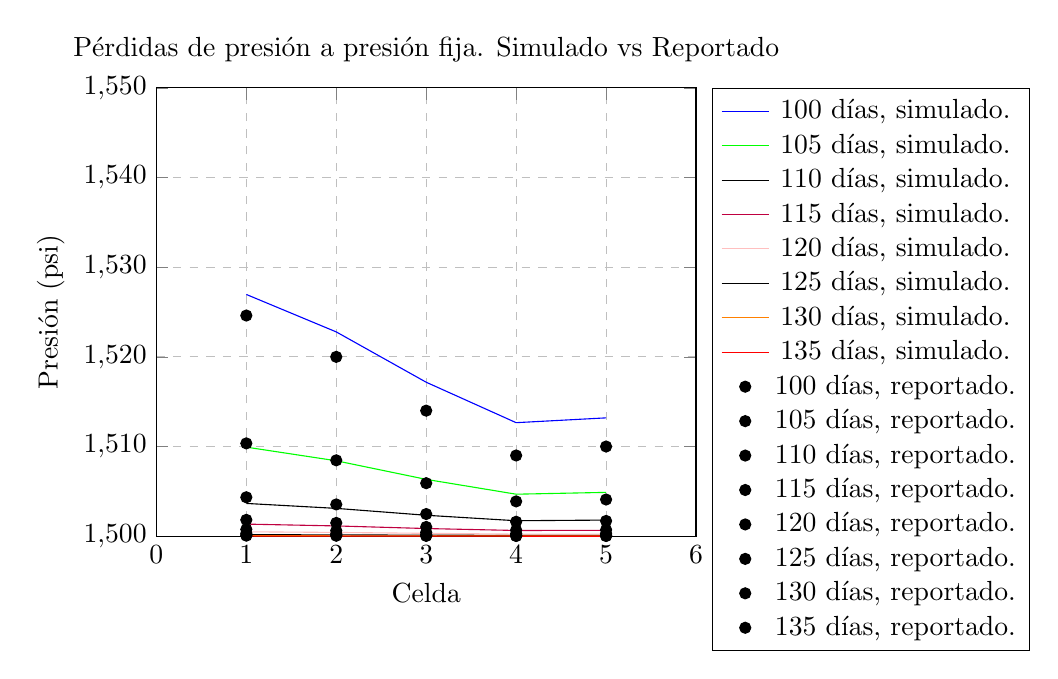
\begin{tikzpicture}
	\begin{axis}[
	title={Pérdidas de presión a presión fija. Simulado vs Reportado},
	xlabel={Celda},
	ylabel={Presión (psi)},
	xmin=0, xmax=6,
	ymin=1500, ymax=1550,
	legend pos=outer north east ,
	ymajorgrids=true,
	xmajorgrids=true,
	%semilogxaxis=true,
	grid style=dashed,
	]
	
	\addplot[color=blue]
	coordinates{
		(1,	1526.960064 )
		(2,	1522.7829696)
		(3,	1517.169999)
		(4,	1512.6593172)
		(5,	1513.1959578)
	};
	\addlegendentry{100 días, simulado.}
	
	\addplot[color=green]
	coordinates{
		(1,	1509.9326028)
		(2,	1508.4097038)
		(3,	1506.3356604)
		(4,	1504.6822272)
		(5,	1504.8852804)
	};
	\addlegendentry{105 días, simulado.}
	
	\addplot[color=black]
	coordinates{
		(1,	1503.6524574)
		(2,	1503.101313)
		(3,	1502.3326116)
		(4,	1501.723452)
		(5,	1501.795971)
	};
	\addlegendentry{110 días, simulado.}
	
	\addplot[color=purple]
	coordinates{
		(1,	1501.3463532)
		(2,	1501.1433)
		(3,	1500.853224)
		(4,	1500.635667)
		(5,	1500.6501708)
	};
	\addlegendentry{115 días, simulado.}
	
	\addplot[color=pink]
	coordinates{
		(1,	1500.490629)
		(2,	1500.41811)
		(3,	1500.3165834)
		(4,	1500.2295606)
		(5,	1500.2295606)
	};
	\addlegendentry{120 días, simulado.}
	
	
	\addplot[]
	coordinates{
		(1,	1500.1715454)
		(2,	1500.1425378)
		(3,	1500.1135302)
		(4,	1500.0845226)
		(5,	1500.0845226)
	};
	\addlegendentry{125 días, simulado.}
	
	\addplot[color=orange]
	coordinates{
		(1,	1500.055515)
		(2,	1500.0410112)
		(3,	1500.0265074)
		(4,	1500.0265074)
		(5,	1500.0265074)
	};
	\addlegendentry{130 días, simulado.}
	
	
	\addplot[red]
	coordinates{
		(1,	1500.0120036)
		(2,	1500.0120036)
		(3,	1500.0120036)
		(4,	1499.9974998)
		(5,	1499.9974998)
	};
	\addlegendentry{135 días, simulado.}
	
	
	\addplot[only marks]
	coordinates{
		(1,	1524.61)
		(2,	1520)
		(3,	1514)
		(4,	1509 )
		(5,	1510)
		
	};
	\addlegendentry{100 días, reportado. }
	
	\addplot[only marks]
	coordinates{
		(1,	1510.35)
		(2,	1508.46)
		(3,	1505.91)
		(4,	1503.88)
		(5,	1504.09)
		
	};
	\addlegendentry{105 días, reportado.}
	
	\addplot[only marks]
	coordinates{
		(1,	1504.34)
		(2,	1503.54)
		(3,	1502.47)
		(4,	1501.61)
		(5,	1501.7)
	};
	\addlegendentry{110 días, reportado. }
	
	\addplot[only marks]
	coordinates{
		(1,	1501.82)
		(2,	1501.48)
		(3,	1501.03)
		(4,	1500.68)
		(5,	1500.71)
	};
	\addlegendentry{115 días, reportado.}
	
	\addplot[only marks]
	coordinates{
		(1,	1500.76)
		(2,	1500.62)
		(3,	1500.43)
		(4,	1500.28)
		(5,	1500.3)
	};
	\addlegendentry{120 días, reportado.}
	
	
	\addplot[only marks]
	coordinates{
		(1,	1500.32)
		(2,	1500.26)
		(3,	1500.18)
		(4,	1500.12)
		(5,	1500.12)
	};
	\addlegendentry{125 días, reportado.}
	
	\addplot[only marks]
	coordinates{
		(1,	1500.13)
		(2,	1500.11)
		(3,	1500.08)
		(4,	1500.05)
		(5,	1500.05)
	};
	\addlegendentry{130 días, reportado.}
	
	
	\addplot[only marks]
	coordinates{
		(1	,1500.06)
		(2	,1500.05)
		(3	,1500.03)
		(4	,1500.02)
		(5	,1500.02)
	};
	\addlegendentry{135 días, reportado.}
	
	\end{axis}
	\end{tikzpicture}
	\caption{Comparativo datos simulados contra caso de estudio de \cite{jamal2006petroleum}. Presión constante.}
	\label{fig:ConstantP}
\end{figure}{}

En la etapa de producción a presión constante se logra observar como la presión del sistema decae hasta que se estabiliza completamente a la presión de abandono. En esta etapa se siguen observando diferencias de alrededor de $10$ $psia$. Con este comportamiento se logra validar el modelo ejecutable para la simulación de casos de producción por flujo natural. Para ejecutar casos en los que se involucren más fenómenos físicos, se requiere un control numérico adicional que no se contempla en el desarrollo de esta Tesis de Maestría.
